\section{Simplex}
Das Simplex ist ein Begriff, welcher aus der Geometrie stammt. Es
beschreibt ein $n$-dimensionales Polytop. Wobei ein Polytop die Bezeichnung
f"ur ein verallgemeinertes Polygon ist, sprich ein verallgemeinertes
Vieleck \cite{bib:link4}. 
Hier einige vorstellbare Beispiele zum Simplex:
 
\begin{center}
\begin{tabular}{c|l}
Dimension & Geometrische Form\\
\hline
$n=0$ & Punkt\\
$n=1$ & Strecke\\
$n=2$ & Dreieck\\
$n=3$ & Tetraeder
\end{tabular}
\end{center}

\begin{figure}
\centering
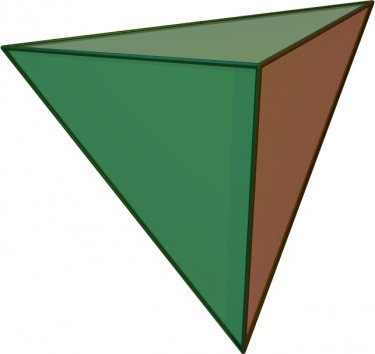
\includegraphics[height=0.25\textwidth]{downhill/tetraeder.jpg}
\caption{Tetraeder als Beispiel eines Simplex f"ur $n=3$}
\end{figure}

Aus der Tabelle wird ersichtlich, dass jedes $n$-dimensionale Simplex genau $n+1$ Ecken hat.
Im Downhill-Simplex-Verfahren wird das Simplex ben"otigt, um die
optimalen Parameterwerte zu finden. Man kann es sich so vorstellen,
dass das Simplex im $n$-dimensionalen Parameterraum aufgespannt wird und
dann f"ur jeden seiner Eckpunkte den entsprechenden Funktionswert (auf
Grund der Zielfunktion) berechnet \cite{bib:link3}.
